\chapter{Content Centric Networking}
\label{chap:ccn}

We now briefly introduce relevant aspects about the Content Centric Networking 
(CCN) paradigm, introduced in Section~\ref{sec:intro-ccnx}.

\section{CCN Packet Types and Content Names}
\label{sec:ccn-packets}

CCN uses two fundamental types of packets: Interest and Data packets (also 
referred to as Content Objects in the scope of Project CCNx~\cite{website:ccnx}, 
a software implementation of the CCN architecture).\vertbreak

\begin{figure}[h!]

    \centering
    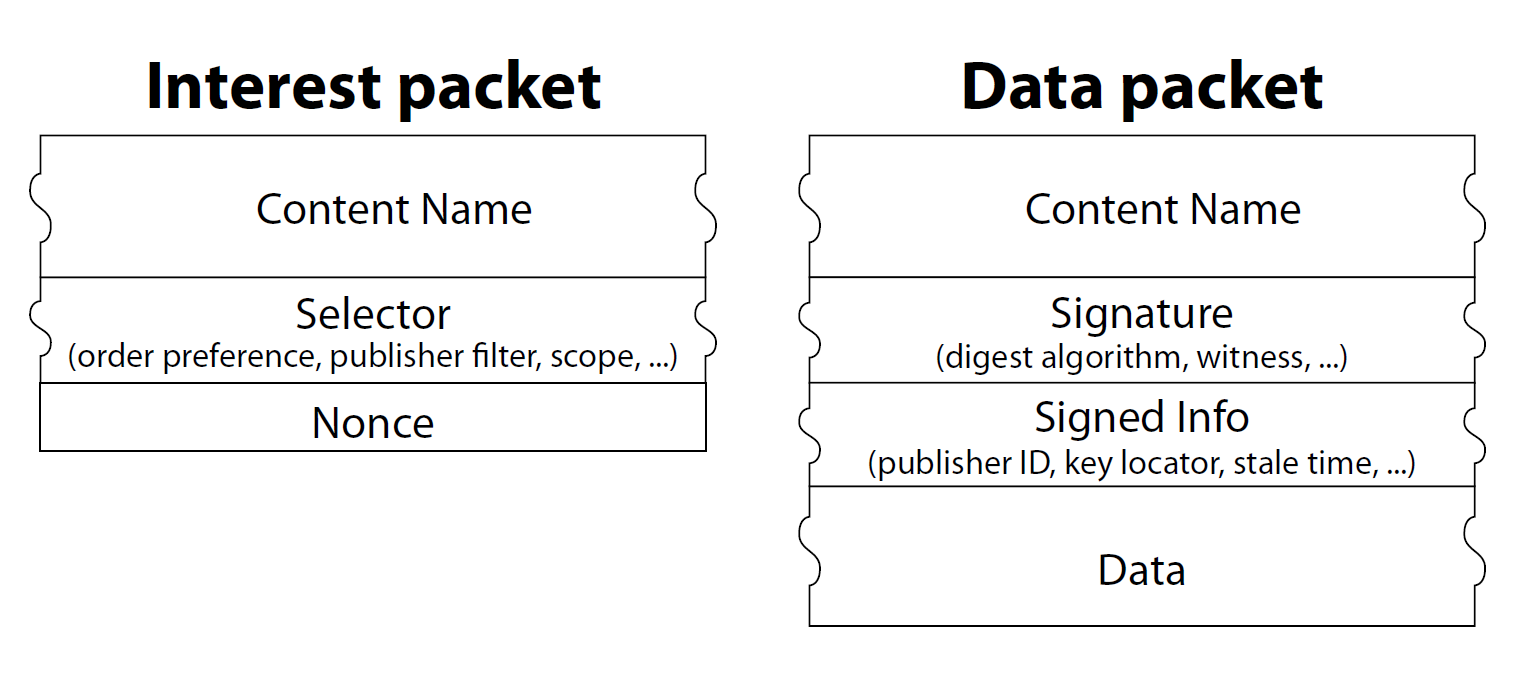
\includegraphics[width=0.65\textwidth]{figures/ccn-packets.png}
    \cprotect\caption{Overview of a CCN Interest and Data packet 
        types~\cite{Jacobson2009}.}
    \label{fig:ccnx-packets}

\end{figure}

Interest packets are originally released into the network by end nodes willing to access a 
particular content, addressing it via its content name. The original paper by 
Jacobson et al.~\cite{Jacobson2009} specifies the use of hierarchical content names, 
e.g. \verb+/sports/football/march.schedule+ (these are also used in practice 
in implementations of CCN, see Section~\ref{subsec:ccnx-specifics}), in order 
to allow publishers to release related content using a single 
prefix and make prefix matching actions intuitive. An Interest packet may 
comprise other fields (e.g. specifying time-limits, maximum number of CCN 
forwarding hops, etc.) and a `nonce' field in order to discard Interest packets 
that may have been duplicated due to network loops (see 
Section~\ref{sec:ccn-forwarding} about CCN forwarding).\vertbreak

Data packets include the content itself with the addition of a cryptographic 
signature. The latter is created by using the data as well as a set of other 
fields such as a timestamp, the publisher's public key (required by other 
nodes to verify signatures), enabling the use of self-certifying names~\cite{Jacobson2009} 
Nodes are supposed to check the signatures and discard any content that fails 
verification.

\section{Forwarding in Content Centric Networks}
\label{sec:ccn-forwarding}

We now introduce the basic forwarding mechanics of a CCN node, starting with 
a description of its inner components.\vertbreak

A CCN node is composed by three main elements: (1) a Forward Information 
Base, (2) a Pending Interest Table (PIT) and (3) a Content Store (CS)~\cite{Jacobson2009}:

\begin{itemize}

    \item \textbf{Forward Information Base (FIB):} Table holding entries 
        which relate a name prefix and a list of interfaces to which 
        Interest packets matching that content name prefix should be forwarded 
        to.
    \item \textbf{Pending Interest Table (PIT):} A table for keeping track of 
        the mapping between arriving Interest packets and 
        the interfaces these have been received from, in order to save a reverse 
        path for Data packets 
        towards one or more subscribers (this may be a 1:N mapping, as an 
        Interest packet matching the same content may be received in 
        multiple interfaces).
    \item \textbf{Content Store (CS):} A cache for content, indexed by Content 
        Name. This is a novel element, allowing for content storage at the 
        Network level. In-network caching allows an Interest to be satisfied 
        by a matching Data packet in any location other than the original 
        producer of the static content, constituting one of the main 
        content-oriented characteristics of CCN.

\end{itemize}

These elements are depicted in Figure~\ref{fig:test-1-1}.\vertbreak

\begin{figure}[h!]

    \centering
    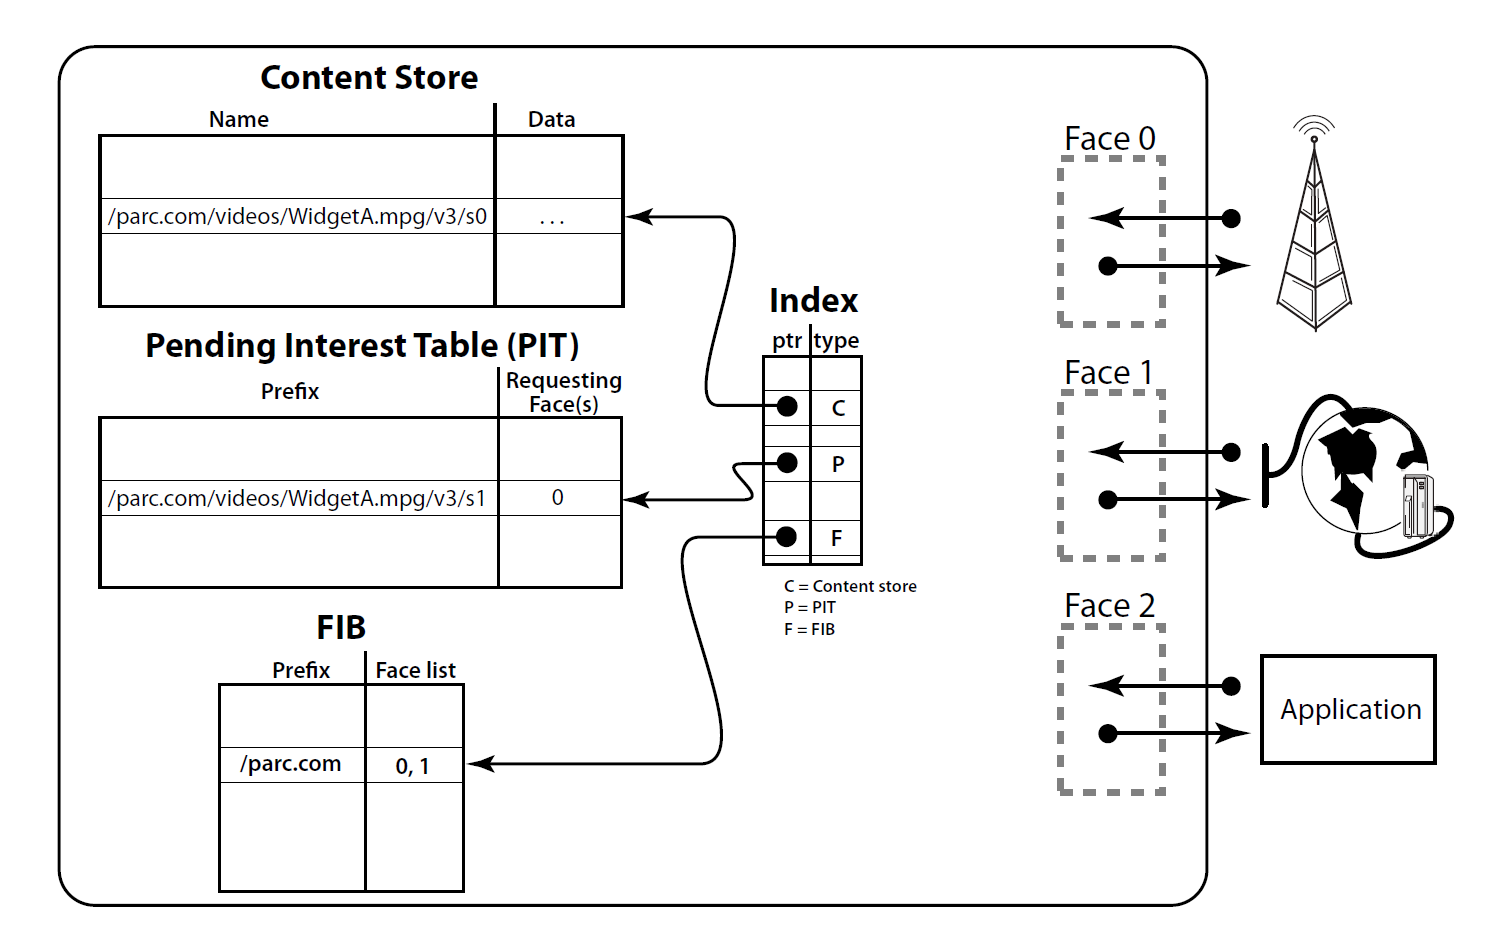
\includegraphics[width=0.65\textwidth]{figures/ccn-node.png}
    \cprotect\caption{Overview of a CCN node's forwarding 
            engine~\cite{Jacobson2009}.}
    \label{fig:test-1-1}

\end{figure}

In CCN, communication is receiver-driven, i.e. having the desire to fetch 
a particular content, an end node releases an Interest packet into the network 
so that it is forwarded towards an appropriate content holder. More precisely, 
an intermediate CCN node performs the following sequence of operations upon the reception of 
an Interest packet~\cite{Jacobson2009}:

\begin{enumerate}

    \item An Interest packet arrives on interface 0 of a given CCN node.
    \item A longest prefix match on the content name specified in the Interest 
        is performed. The CCN node will now look in its CS, PIT and FIB, in 
        that order, in order to resume the forwarding action:
        \begin{enumerate}

            \item If there's a match on the node's CS, a copy of the respective 
                CS entry will be sent back via interface 0, the Interest 
                packet is dropped. \textbf{End.}

            \item Else if there is an (exact) match on the PIT, interface 0 is 
                added to the mapping list on the respective entry. The 
                Interest packet is dropped (as a previous one has already been 
                sent upstream). \textbf{End.}

            \item Else if only a matching FIB entry is found, the Interest 
                packet is forwarded upstream, via all remaining interfaces on the 
                list (other than 0), towards an eventual content holder. A PIT 
                entry $<$content name, interface 0$>$ is added. \textbf{End.}

            \item Else if there is no match at all, the Interest packet is 
                simply discarded. \textbf{End.}

        \end{enumerate}

\end{enumerate}

Note that in CCN 
only Interest packets are routed: as the intermediate CCN nodes forward the 
Interests, their respective PIT tables are updated with Interest-to-interface 
mappings, pre-establishing a reverse path for Data packets to follow as a 
content holder is found. When the reverse path is started by a CCN node 
holding a particular content name, each intermediate CCN node receiving a 
Data packet looks in its PIT for $<$content name, interface n$>$ entries, 
and forwards the Data packet through all matching interfaces. In addition, a 
CS entry is created to cache the content locally at the node. If a Data packet 
with no matching PIT entries arrives, it is treated as unsolicited and discarded.
